\documentclass[tikz,border=10pt]{standalone}
\usepackage{ctex} % 支持中文（如有需要）
\usetikzlibrary{calc, intersections}

\begin{document}

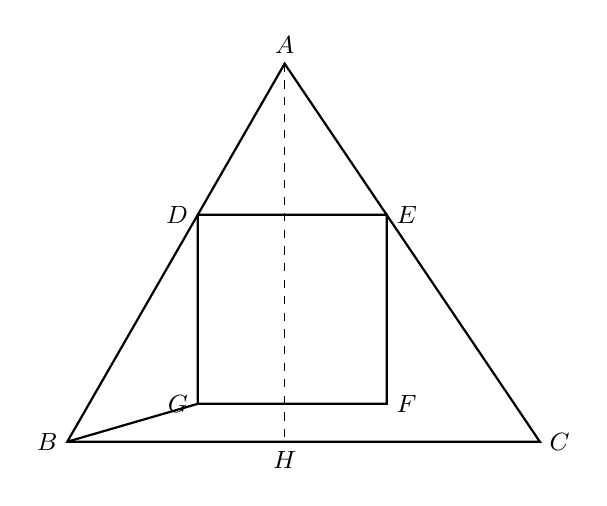
\begin{tikzpicture}[>=latex, font=\small, scale=1.2]
    % --- 1. 定义关键点坐标 ---
    % 定义大三角形的顶点
    \coordinate (A) at (2.3, 4);
    \coordinate (B) at (0, 0);
    \coordinate (C) at (5, 0);
    
    % --- 2. 绘制大三角形 ABC ---
    \draw[thick] (A) -- (B) -- (C) -- cycle;
    
    % --- 3. 计算并绘制矩形/正方形 DEFG ---
    % 设定矩形的高度比例或固定高度，此处根据原图比例取值
    % D, E 分别在 AB 和 AC 上，DE 平行于 BC
    \coordinate (D) at ($(A)!0.4!(B)$);
    \coordinate (E) at ($(A)!0.4!(C)$);
    
    % 计算下方顶点 G, F (垂足方向)
    % G, F 在本图中并非全部落在 BC 上，而是悬空形成闭合框
    \coordinate (G) at ($(D) + (0, -2)$);
    \coordinate (F) at ($(E) + (0, -2)$);
    
    % 绘制矩形 DEFG
    \draw[thick] (D) -- (E) -- (F) -- (G) -- cycle;
    
    % --- 4. 绘制辅助线 ---
    % 绘制高 AH (过 A 垂直于 BC)
    \coordinate (H) at (2.3, 0);
    \draw[dashed, thin] (A) -- (H);
    
    % 绘制连线 BG
    \draw[thick] (B) -- (G);
    
    % --- 5. 标注文本标签 ---
    % 锚点设定保证标签不遮挡线条
    \node[above] at (A) {$A$};
    \node[left]  at (B) {$B$};
    \node[right] at (C) {$C$};
    \node[left]  at (D) {$D$};
    \node[right] at (E) {$E$};
    \node[left]  at (G) {$G$};
    \node[right] at (F) {$F$};
    \node[below] at (H) {$H$};
    
\end{tikzpicture}

\end{document}